\chapter{Detekcia objektov v obraze}

    Pre niektoré techniky klasifikácie objektov je nutné najprv v obraze tieto objekty nájsť. Existuje k tomu veľké množstvo metodík, pri čom každá z nich má svoje výhody a nevýody. Je teda nutnosťou zistiť ktorá metóda najviac vyhovuje použitiu pre túto prácu.

\section{Prahovanie}

    Prahovanie je jasová transformácia pri ktorej je šedotónový obraz rozdelený na dve a viac oblastí podľa jasovej úrovne pixelov. O tom, do ktorej z oblastí je daný pixel priradený rozhoduje prah, ktorého hodnotu je treba určiť. Výsledkom je obraz s len dvomi úrovňami jasu - binárny obraz.

    Pri správnom predspracovaní obrazu prahovaním, je možné v ňom jednoducho oddeliť objekty od pozadia, v prípade ak sa jas objektu dostatočne lýši od jasu pozadia. Ak sa však jasové hodnoty objektu a pozadia príliš podobajú, nemusí existovať dostatočne robustné určenie prahu oddeľujúceho objekty od pozadia.

    \begin{figure}[!ht]
        \begin{center}
            \includegraphics[scale=.4]{obrazky/threshold/thresholding.png}
        \end{center}
        \caption{Funkcia prahovania s prahom 0.5 pre svetlé pozadie}
    \end{figure}

\subsection{Globálne prahovanie}

    Globálne prahovanie je často používaná technika pri ktorej je použítý jediný prah na celý obraz, čo nemusí byť vhodné v prípade ak je jasová úroveň pozadia rôzna v rôznych miestach obrazu.

    \begin{itemize}
        \item \textbf{Jednoduché prahovanie} je technika pri ktorej je globálny prah určený dopredu ručne. V prípade že sa jasová úroveň pozadia v čase mení, je vhodnejšie použiť techniky s adaptívnym nastavením prahu.

        \item Prahovanie \textbf{podľa známeho rozloženia} predpokladá že poznáme relatívnu veľkosť oblasti ktorú zaberá pozadie v obraze. Ak vieme že objekt je svetlejší ako pozadie, môžeme určiť prah z kumulatívneho histogramu tak, aby relatívny počet pixelov pod úrovňou prahu bol rovnaký ako oblasť ktorú ma zaberať pozadie.

        \item Algoritmus \textbf{K-Means} (K priemerov) pre zhlukovú analýzu, rozdeľuje dáta do skupín s cieľom minimalizovať vzdialenosť bodov v zhluku a maximalizovať vzdialenosť medzi zhlukmi. Jedná sa o algorytmus učenia bez učiteľa. Funguje na princípe iterovaného posúvania \emph{k} stredov zhlukov (v prípade binárneho prahovania je \emph{k = 2}), smerom k priemeru hodnôt priradenému danému stredu v aktuálnom kroku.

        \item \textbf{Otsuova metóda} automatického určenia prahu je založená na maximalizovaní vzájomnej odchýlky medzi triedami. Využíva normalizovaný kumulatívny histogram z ktorého určuje vzájomnú rozptyl pre všetky možné hodnoty prahu a vyberá ten optimálny. 
    \end{itemize}

    \begin{figure}[!ht]
        \centering
        \begin{tikzpicture}[>=stealth, node distance=5cm]
            \node (image1) {\includegraphics[width=.3\textwidth]{obrazky/threshold/img.png}};
            \node (image2) [right of=image1] {\includegraphics[width=.3\textwidth]{obrazky/threshold/img_gray.png}};
            \node (image3) [right of=image2] {\includegraphics[width=.3\textwidth]{obrazky/threshold/img_simple_thresh.png}};

            \draw[->] (image1) -- (image2) node[midway, above] {};
            \draw[->] (image2) -- (image3) node[midway, above] {};
        \end{tikzpicture}
        \begin{tikzpicture}[>=stealth, node distance=5cm]
            \node (image1) {\includegraphics[width=.3\textwidth]{obrazky/threshold/img_dark.png}};
            \node (image2) [right of=image1] {\includegraphics[width=.3\textwidth]{obrazky/threshold/img_dark_gray.png}};
            \node (image3) [right of=image2] {\includegraphics[width=.3\textwidth]{obrazky/threshold/img_dark_simple_thresh.png}};

            \draw[->] (image1) -- (image2) node[midway, above] {};
            \draw[->] (image2) -- (image3) node[midway, above] {};
        \end{tikzpicture}
        \caption{Jednoduché prahovanie}
    \end{figure}

    \begin{figure}[!ht]
        \centering
        \begin{tikzpicture}[>=stealth, node distance=5cm]
            \node (image1) {\includegraphics[width=.3\textwidth]{obrazky/threshold/img.png}};
            \node (image2) [right of=image1] {\includegraphics[width=.3\textwidth]{obrazky/threshold/img_gray.png}};
            \node (image3) [right of=image2] {\includegraphics[width=.3\textwidth]{obrazky/threshold/img_thresh_distr.png}};

            \draw[->] (image1) -- (image2) node[midway, above] {};
            \draw[->] (image2) -- (image3) node[midway, above] {};
        \end{tikzpicture}
        \begin{tikzpicture}[>=stealth, node distance=5cm]
            \node (image1) {\includegraphics[width=.3\textwidth]{obrazky/threshold/img_dark.png}};
            \node (image2) [right of=image1] {\includegraphics[width=.3\textwidth]{obrazky/threshold/img_dark_gray.png}};
            \node (image3) [right of=image2] {\includegraphics[width=.3\textwidth]{obrazky/threshold/img_thresh_distr.png}};

            \draw[->] (image1) -- (image2) node[midway, above] {};
            \draw[->] (image2) -- (image3) node[midway, above] {};
        \end{tikzpicture}
        \caption{Automatické prahovanie (podľa známeho rozloženia)}
    \end{figure}

\subsection{Lokálne prahovanie}

    V prípade že je jas pozadia rôzny v rôznych častiač obrazu, je vhodné určiť hodnotu prahu z jasovej úrovne okolia každého prahovaného pixelu. Toto takzvané adaptívne prahovanie, má síce vyžšiu výpočetnú náročnosť ako jednoduchšie globálne prahovanie, keďže je nutné určiť prah pre každý bod obrazu samostatne, je však robustnejšie voči nevhodnému pozadiu.

    \begin{figure}[!ht]
        \centering
        \begin{tikzpicture}[>=stealth, node distance=5cm]
            \node (image1) {\includegraphics[width=.3\textwidth]{obrazky/threshold/img2.png}};
            \node (image2) [below of=image1] {\includegraphics[width=.3\textwidth]{obrazky/threshold/img2_gray.png}};
            \node (image3) [left of=image2] {\includegraphics[width=.3\textwidth]{obrazky/threshold/img2_simple_thresh.png}};
            \node (image4) [right of=image2] {\includegraphics[width=.3\textwidth]{obrazky/threshold/img2_adaptive_thresh.png}};

            \draw[->] (image1) -- (image2) node[midway, above] {};
            \draw[->] (image2) -- (image3) node[midway, above] {};
            \draw[->] (image2) -- (image4) node[midway, above] {};
        \end{tikzpicture}
        \caption{Adaptívne prahovanie (podľa známeho rozloženia)}
    \end{figure}

\section{Detekcia hrán}

    Ako jednu z metód vyhľadávania objektov v obraze je možné využiť obraz hrán a vyhľadať v ňom kontúry objektov. Opäť existuje niekoľko spôsobov ako získať obraz hrán a ako ho využiť k segmentácii obrazu, teda k detekcii objektov.

    Na vytvorenie obrazu hrán z nasnímaného obrazu sa používa konvolúcia obrazu s operátorom navrhnutým tak aby aproximovalo deriváciu určitého rádu. Medzi často používané operátory patria Prewittov a Sobelov operátor, ktoré aproximujú prvú deriváciu v určitom smere (horizontálnom, vertikálnom, diagonálne). Druhú deriváciu aproximuje Laplaceov operátor, používa sa tiež v kombinácii s Gaussovým filtrom (LoG operátor), čo má za následok zníženie citlivosti na šum.

    % konvolučné operátory - hranové detektory
    \begin{figure}[!ht]
        \centering

        \begin{minipage}[b]{0.2\textwidth}
            \[
                \begin{bmatrix}
                    -1 & 0 & 1 \\
                    -1 & 0 & 1 \\
                    -1 & 0 & 1 \\
                \end{bmatrix}
            \]
            \centering
            Prewittov operátor
        \end{minipage}
        %
        \begin{minipage}[b]{0.2\textwidth}
            \[
                \begin{bmatrix}
                    -1 & 0 & 1 \\
                    -2 & 0 & 2 \\
                    -1 & 0 & 1 \\
                \end{bmatrix}
            \]
            \centering
            Sobelov operátor
        \end{minipage}
        %
        \begin{minipage}[b]{0.2\textwidth}
            \[
                \begin{bmatrix}
                    0 &  1 & 0 \\
                    1 & -4 & 1 \\
                    0 &  1 & 0 \\
                \end{bmatrix}
            \]
            \centering
            Laplaceov operátor
        \end{minipage}
        
        \begin{minipage}[b]{0.4\textwidth}
            \[
                \begin{bmatrix}
                    0 & 0 & -1 & 0 & 0 \\
                    0 & -1 & -2 & -1 & 0 \\
                    -1 & -2 & 16 & -2 & -1 \\
                    0 & -1 & -2 & -1 & 0 \\
                    0 & 0 & -1 & 0 & 0 \\
                \end{bmatrix}
            \]
            \centering
            LoG operátor
        \end{minipage}
    \end{figure}

    Komplexnejšiou metódou detekcie hrán je takzvaný \emph{Cannyho hranový detektor}. Ide o proces vo viacerých krokoch, pre jeden vstupný obraz sa postupuje nasledovne:

    \begin{enumerate}
        \item Vstupný obraz býva väčšinou filtrovaný z dôvodu zníženia citlivosti na šum v obraze. Vhodné je k tomu napríklad Gaussove rozmazanie.
        
        \item Použije sa horizontálny a vertikálny Sobelov operátor ako detektor hrán, na získanie obrazu hrán v oboch smeroch \(I_{x}\) a \(I_{y}\).

        \begin{minipage}[b]{0.4\textwidth}
            \[I_{x} = 
            \begin{bmatrix}
                -1 & 0 & 1 \\
                -2 & 0 & 2 \\
                -1 & 0 & 1 \\
            \end{bmatrix}
            \ast I
            \]
        \end{minipage}
        %
        \begin{minipage}[b]{0.4\textwidth}
            \[I_{y} = 
            \begin{bmatrix}
                 1 &  2 &  1 \\
                 0 &  0 &  0 \\
                -1 & -2 & -1 \\
            \end{bmatrix}
            \ast I
            \]
        \end{minipage}

        \item Z toho je možné určiť magnitúdu a smer gradientu:
        
        \begin{minipage}[b]{0.4\textwidth}
            \[G = \sqrt{I_x^2 + I_y^2}\]
        \end{minipage}
        \begin{minipage}[b]{0.4\textwidth}
            \[\theta = atan2(I_x, I_y)\]
        \end{minipage}
        
        \item Ku zníženiu redundancie detekovaných hrán sa použije algorytmus \emph{non maxima suppression} (potlačenie nemaximálnej hodnoty). Použitím tohoto algorytmu dôjde k zúženiu hrán, pričom sa ponechajú len tie časti hrán ktorých magnitúda je väčšia ako v ich okolí.
        
        \item Dvojitým prahovaním sa v obraze hrán nájdu tri úrovne:
            \begin{itemize}
                \item \textbf{silné hrany} sú hrany vyššie ako obidva prahy. Do výsledného obrazu hrán sú určite pridané.
                \item \textbf{slabé hrany} sú hrany medzi dvomi prahmi.
                \item \textbf{nie hrany} sú tie hrany ktorých magnitúda je nižšia ako obidva prahy.
            \end{itemize}
            
        \item Iteratívne sú slabé hrany dotýkajúce sa silných hrán označované za silné, až kým sa žiadna slabá hrana silnej nedotýka. Vo výslednom obraze sú ponechané len silné hrany.
    \end{enumerate}

    \begin{figure}[!ht]
        \centering
        \begin{tikzpicture}[>=stealth, node distance=5cm]
            \node (image1) {\includegraphics[width=.3\textwidth]{obrazky/canny/img.png}};
            \node (image2) [right of=image1] {\includegraphics[width=.3\textwidth]{obrazky/canny/img_gray.png}};
            \node (image3) [right of=image2] {\includegraphics[width=.3\textwidth]{obrazky/canny/img_gauss.png}};
            \node (image4) [below of=image2] {\includegraphics[width=.3\textwidth]{obrazky/canny/img_sobel_x.png}};
            \node (image5) [right of=image4] {\includegraphics[width=.3\textwidth]{obrazky/canny/img_sobel_y.png}};
            \node (image6) [below of=image5] {\includegraphics[width=.3\textwidth]{obrazky/canny/img_mag.png}};
            \node (image7) [left of=image6] {\includegraphics[width=.3\textwidth]{obrazky/canny/img_nms.png}};
            \node (image8) [left of=image7] {\includegraphics[width=.3\textwidth]{obrazky/canny/img_double_thresh.png}};
            \node (image9) [above of=image8] {\includegraphics[width=.3\textwidth]{obrazky/canny/img_canny.png}};

            \draw[->] (image1) -- (image2) node[midway, above] {};
            \draw[->] (image2) -- (image3) node[midway, above] {};
            \draw[->] (image3) -- (image4) node[midway, above] {};
            \draw[->] (image3) -- (image5) node[midway, above] {};
            \draw[->] (image4) -- (image6) node[midway, above] {};
            \draw[->] (image5) -- (image6) node[midway, above] {};
            \draw[->] (image6) -- (image7) node[midway, above] {};
            \draw[->] (image7) -- (image8) node[midway, above] {};
            \draw[->] (image8) -- (image9) node[midway, above] {};
        \end{tikzpicture}
        \caption{Cannyho hranový detektor}
    \end{figure}

    Obraz hrán je možné ďalej spracovávať, napríklad morfologickýmy operáciami: otvorením odstrániť krátke nevýznamné hrany, zatvorením spojiť hrany blízko pri sebe.

    Vyhľadávaním uzavertých kontúr v obraze hrán je možné identifikovať potenciálne objekty v obraze.

    \subsection{Detekcia horizontu pomocou Houghovej transformácie}

        Pokiaľ časť obrazu obsahuje horizont, je vhodnejšie detekovať lietajúce objekty len na oblohe nad ním, aby sa predišlo falošným detekciám. Horizont je možné detekovať z obrazu hrán pomocou Houghovej transformácie, podľa práce. Vo výsledku Houghovej transformácie sa horizont prejaví ako najvýraznejšia čiara.


        \begin{figure}[H]
            \centering
            \begin{tikzpicture}[>=stealth, node distance=8cm]
                \node (image1) {\includegraphics[width=.4\textwidth]{obrazky/canny/img_canny.png}};
                \node (image2) [below of=image1, yshift=2.5cm] {\includegraphics[width=.45\textwidth]{obrazky/canny/img_hough.png}};
                \node (image3) [right of=image2] {\includegraphics[width=.4\textwidth]{obrazky/canny/img_horizon.png}};

                \draw[->] (image1) -- (image2) node[midway, above] {};
                \draw[->] (image2) -- (image3) node[midway, above] {};
            \end{tikzpicture}
            \caption{Detekcia horizontu pomocou Houghovej transformácie}
        \end{figure}

\section{Detekcia pohybu}

    V prípade že je požadovaná detekcia pohybujúcich sa objektov, je možnosťou detekcie práve detekovaním ich pohybu. Jednou z jednoduchých metód detekcie pohybu sú rozdielové metódy, pri ktorých je vypočítavaný rozdielový snimok z viacerých snímkov zo sekvencie \(\{I_1, I_2, ..., I_n\}\). Rozdielový snímok môže byť:

    \begin{itemize}
        \item \textbf{jednostranný} - je najjednoduchší nenesie informáciu o smere pohybu, vyhodnocuje sa len v miestach kde \(I_1(x,y) > I_2(x,y)\).
        \[D(x,y) = \begin{cases}
            0 & I_1(x,y) - I_2(x,y) < \epsilon \\
            1 & I_1(x,y) - I_2(x,y) \geq \epsilon
        \end{cases}\]

        \item \textbf{obojstranný} - dostaneme ho upravením vzťahu pre jednostranný rozdielový snímok, použitím absolútnej hodnoty. Tým je dosiahnutá zameniteľnosť \(I_1(x,y)\) a \(I_2(x,y)\), vyhodnocuje sa teda na celom obraze. Neodstraňuje nedostatok informácie o smere pohybu, tá však nemusí byť nutnosťou.
        \[D(x,y) = \begin{cases}
            0 & |I_1(x,y) - I_2(x,y)| < \epsilon \\
            1 & |I_1(x,y) - I_2(x,y)| \geq \epsilon
        \end{cases}\]

        \item \textbf{kumulovaný} - je vytvorený váženým súčtom jedno alebo obojstranných rozdielových snímkov. Je teda možné priemerovať pohyb za určitý čas určením každej váhy \(\omega = 1/(N-1)\), alebo určiť rôznym snímkom rôznu váhu a získať tak informáciu o smere pohybu.
        \[D(x,y) = \sum_{i=1}^{N-1}\omega_i \cdot D_i(x,y)\]
    \end{itemize}

    Komplexnejšiou metódou detekcie pohybu je vytvorenie rozdielového snímku nie medzi nasledujúcimi snímkami, ale aktuálnym snímkom a vytvoreným modelom pozadia. Ten je možné zostaviť:

    \begin{itemize}
        \item ako jeden obraz pozadia bez objektov.
        \item ako priemerný snímok niekoľkých snímkov pozadia.
        \item ako dynamický model - iteratívnym aktualizovaním podľa aktuálneho snímku. Tým sa model pozadia postupne prispôsobuje malým zmenám v prostredí.
    \end{itemize}

    \begin{figure}[H]
        \centering
        \begin{tikzpicture}[node distance=.3cm, auto]

            % Define block styles
            \tikzstyle{block} = [rectangle, draw, fill=white!20, text width=12em, text centered, sharp corners, minimum height=4em]
            \tikzstyle{line} = [draw, -latex']

            % Nodes
            \node [block] (start) {prejdi na ďalší snímok
            
            i \(\leftarrow\) i + 1};
            \node [block, below=of start] (calc_d1) {výpočet \(D_1(x,y)\) medzi \(I_i(x,y)\) a \(I_{i-1}(x,y)\)};
            \node [draw, diamond, aspect=4, below=of calc_d1] (check_d1) {vykazuje \(D_1(x,y)\) významný pohyb?};
            \node [block, below=of check_d1] (calc_d2) {vypočítaj \(D_2(x,y)\) medzi \(I_i(x,y)\) a \(B_i(x,y)\)};
            \node [draw, diamond, aspect=4, below=of calc_d2] (check_d2) {vykazuje \(D_2(x,y)\) významný pohyb?};
            \node [block, below=of check_d2] (calc_b) {vypočítaj \(B_{i+1}(x,y)\)};

            % Arrows
            \path [line] (start) -- (calc_d1);
            \path [line] (calc_d1) -- (check_d1);
            \path [line] (check_d1.west) -- ++(0,2.75) -- node [below = .3cm] {áno} (start.190);
            \path [line] (check_d1) -- node [near start] {nie} (calc_d2);
            \path [line] (calc_d2) -- (check_d2);
            \path [line] (check_d2.west) -- ++(-1,1) -- ++(0,7) -- node [near start] {áno} (start.170);
            \path [line] (check_d2) -- node [near start] {nie} (calc_b);
            \path [line] (calc_b.east) -- ++(3,1) -- ++(0,9) -- (start.east);

        \end{tikzpicture}
        \caption{Postup aktualizovania dynamického modelu pozadia}
    \end{figure}

    Výpočet nového modelu pozadia \(B_{i+1}(x,y)\) môže prebiehať napríklad pomocou lineárneho zabúdania, teda \(B_{i+1}(x,y) = \alpha \cdot I_i(x,y) + (1 - \alpha) \cdot B_i(x,y)\).

    Obraz obsahujúci detekovaný pohyb je získaný rozdielom a prahovaním aktuálneho snímku a modelu pozadia.

    \begin{figure}[H]
        \centering
        \begin{tikzpicture} [node distance=1.5cm, auto]
            \node (image1) {\includegraphics[width=.3\textwidth]{obrazky/motion/frame.png}};
            \node (space1) [below of=image1] {};
            \node (image2) [below of=space1] {\includegraphics[width=.3\textwidth]{obrazky/motion/background.png}};
            \node (sum) [draw, rectangle, right of=space1, xshift=2.5cm] {D(x,y)};
            \node (threshold) [draw, rectangle, right of=sum, xshift=.5cm] {\(\geq \epsilon\)};
            \node (image3) [right of=threshold, xshift=2.5cm] {\includegraphics[width=.3\textwidth]{obrazky/motion/motion.png}};

            \draw[->] (image1.east) to [out=0, in=90] (sum.north);
            \draw[->] (image2.east) to [out=0, in=270] (sum.south);
            \draw[->] (sum) -- (threshold);
            \draw[->] (threshold) -- (image3);
        \end{tikzpicture}
        \caption{Odčítanie pozadia}
    \end{figure}

\chapter{Popis objektov}

    \section{príznaky}

\chapter{Klasifikácia}

    Ďalším krokom je určenie triedy detekovaných objektov, teda ich klasifikácia. Tá môže byť vykonaná na základe obrazu, alebo pomocou príznakov získaných z neho.

    \section{Konvolučné neurónové siete}

        Na rozdiel od plne prepojenej neurónovej siete, sú \ac{CNN} prispôsobené na prácu s obrazom ako so vstupným signálom. Ich architektúra je usporiadaná do vrstiev, štandardne po sebe nasledujú:

        \begin{enumerate}
            \item \textbf{Konvolučná vrstva} - používa konvolučné filtre na extrakciu príznakov z obrazu.
            \item \textbf{Aktivačná vrstva} - aplikuje aktivačnú funkciu, často napríklad \ac{ReLU} na každý bod. Zavádza do siete nelinearitu a pomáha zachytávať zložitejšie vzory.
            \item \textbf{Pooling vrstva} - redukuje priestorové rozlíšenie vstupných dát. Tým sa zníži výpočtová náročnosť nasledujúcich vrstiev. Najčastejšie sa používa \emph{max pooling}, teda výber najvyššej hodnoty v okolí.
        \end{enumerate}

        Väčšinou je použitá kombinácia niekoľko \textbf{konvolučných} vrstiev nasledovaných \textbf{aktivačnou} vrstvou, po ktorých \textbf{pooling} vrstva pripraví redukovaný vstup pre ďalšie vrstvy. Takýchto kombinácii nasleduje niekoľko, posledná je pripojená na plne prepojenú neurónovú sieť. Konvolučná časť slúži na vyhľadávanie príznakov, plne prepojená časť na klasifikáciu pomocou nich.

        \begin{figure}[h]
            \centering
            \includegraphics[width=.9\textwidth]{obrazky/cnn/cnn.png}
            \caption{Príklad architektúry konvolučnej neurónovej siete}
        \end{figure}

        Rozmery vrstiev závisia na tvare vstupného signálu. V prípade šedotónového obrazu je každý bod obrazu reprezentovaný jednou skalárnou hodnotou, v prípade farebného záleží počet hodnôt na pixel na farebnom modele. Klasifikáciou z farebného obrazu získavame väčšie množstvo informácii ale je vyžadovaný vyšší výkon, nakoľko sa konvolučné filtre aplikujú po jednom na každú zložku obrazu (teda v prípade RGB modelu na červenú, zelenú a modrú zložku samostatne).

        Výstup z poslednej vrstvy plne prepojenej časti siete je výstupom z celej \ac{CNN}. Výstupy klasifikačnej neurónovej siete s úlohov klasifikovať viacero tried, mávajú formáty:

        \begin{itemize}
            \item Jeden výstup, ktorého hodnota určuje triedu do ktorej sú vstupné dáta sieťou priradené.
            \item Vektor výstupov výstupov s toľkými hodnotami, na koľko tried je naučená sieť klasifikovať. Hodnoty výstupov môžu reprezentovať:
            \begin{itemize}
                \item Ohodnotenie triedy (score-based classification). V tomto prípade čísla na výstupe nemajú samostatne význam, ale ako predpoveď je určená trieda s najvyšším skóre.
                \item Pravdepodobnosť zaradenia do danej triedy. Tá je získaná použitím výstupnej aktivačnej vrstvy typu \emph{softmax}, ktorá spôsobí že každý z výstupov má hodnotu od 0 do 1 a súčet všetkých výstupov je 1.
            \end{itemize}
        \end{itemize}
        

\chapter{Detekcia a klasifikácia v jednom kroku}

    \section{R-CNN}

        \ac{R-CNN} sú skupina modelov strojového učenia zaločená na \ac{CNN}. Ich cieľom je nájdenie a klasifikovanie objektov v obraze. Ich výstupom je množina rámčekov ohraničujúcich objekty a im pridelené triedy.

        \ac{R-CNN} pracujú v niekoľkých etapách:
        \begin{enumerate}
            \item \textbf{Selektívne vyhľadávanie} - vstupný obraz je spracovaný a sú extrahované \ac{RoI}, teda orámované oblasti obrazu, ktoré by mohli obsahovať objekty alebo ich časti. Počet takto navrhovaných oblastí môže dosahovať niekoľko tisíc.
            \item \textbf{Extrakcia príznakov} - každý \ac{RoI} je predložený ako vstup pre naučenú \ac{CNN}, ktorá vyprodukuje príznakový vektor pre každý \ac{RoI}.
            \item \textbf{Klasifikácia} - pomocou skupiny modelov \ac{SVM} je podľa príznakov extrahovaných \ac{CNN}, klasifikovaný každý \ac{RoI} do jednej z určených tried alebo ako pozadie - teda nepatriaci do žiadnej triedy.
            \item \textbf{Regresia ohraničení} - konečný krok, zvyšujúci presnosť orámovania objektov. Používa sa pri ňom naučený model nezávyslý na mierka nazývaný \emph{bounding box regressor}. Jeho výstup je štvorrozmerný, skladá sa z polohy a rozmerov ohraničujúceho obdĺžnika.
        \end{enumerate}

        \ac{R-CNN} sú efektívne, no náročné na výpočetný výkon. Z toho dôvodu boli vyvinuté rýchlejšie varianty \emph{Fast R-CNN} a \emph{Faster R-CNN}.

        \emph{Fast R-CNN} aplikuje \ac{CNN} na celý vstupný obraz a extrahuje z neho mapu príznakov. Až na výslednú mapu aplikuje takzvaný \ac{RoI} \emph{pooling}, ktorý extrahuje príznaky pre každý \ac{RoI}, pomocou okna pevnej veľkosti. Zvyšok modelu pracuje podobne ako \ac{R-CNN}, s využitím plne prepojenej siete na klasifikáciu a generovanie orámovaní.

        \emph{Faster R-CNN} nadväzuje na \emph{Fast R-CNN} nahradením selektívneho vyhľadávania modelom typu \ac{RPN}. Vstupný obraz prechádza predučenou \ac{CNN}, sú extrahované príznaky. \ac{RPN} využije nájdené príznaky aby určila kde sa nachádzajú potenciálne objekty v obraze. V konečnom kroku sú klasifikované navrhnuté ohraničené oblasti podľa príznakov extrahovaných v predošlom kroku. \emph{Faster R-CNN} je dostatočne rýchla na použitie v reálnom čase.

    \section{YOLO}

        \ac{YOLO} je populárny algorytmus detekcie, ktorý na rozdiel od \ac{R-CNN} rozdeľuje obraz do mriežky a postupne aplikuje klasifikátor. Postupuje nasledovne:

        \begin{enumerate}
            \item Vstuný obraz je rozdelený na mriežku \(S \times S\), ktorej veľkosť závisí na verzii \ac{YOLO}.
            \item V každej bunke mriežky je predikovaný určitý počet ohraničených oblastí a im priradené skóre dôveryhodnosti. Tie značia úroveň istoty že oblasť obsahuje objekt a že dané ohraničenie je správne.
            \item Je použitých viacero klasifikátorov. \ac{YOLO} predikuje viacero oblastí za každú bunku. Počas trénovania je jednému z prediktorov udelená zodpovednosť za predikovanie daného objekto podľa toho ktorý z nich dosahuje najväčší \ac{IOU}.
            \item Každá bunka predikuje rozdelenie pravdepodobnosti všetkých tried.
        \end{enumerate}

        Hlavnou výhodou \ac{YOLO} je rýchlosť. Všeobecne pracuje rýchlejšie a s menším požadovaným výpočetným výkonom. Na druhú stranu má nevýhody spôsobené obmedzením veľkosti orámovaných oblastí. Presnosť \ac{YOLO} býva nižšia pri primalých objektoch, pre použitia vyžadujúce vyžšiu presnosť sa môže javiť ako výhodnejšie použiť iné modely.

\chapter{Návrh kombinácie a usporiadania hardvérových komponentov}

    Táto kapitola sa zameriava na návrh a implementáciu prenosného zariadenia pre detekciu, klasifikáciu a trasovanie lietajúcich objektov. Cieľom návrhu je vytvorenie zariadenia s možnosťou nasadenia v čo najrôznejších podmienkach. Jednou z podminok je teda jeho prenosnosť, možnosť napájania z akumulátoru a nezávyslosť na iných zariadeniach pri jeho nastavení a používaní.

    \section{Jednodoskový počítač}
    
        Jedným z najčastejšie používaných jednodoskových počítačov je rada \emph{Raspberry Pi}. V čase návrhu bol najnovším model \emph{Pi 4 model B}. Tento model disponuje:
        \begin{itemize}
            \item 1.5GHz ARM Cortex-A72 procesorom so 4 jadrami,
            \item do 8 Gb pamäte RAM,
            \item rozhraním HDMI s možnosťou pripojenia dvoch monitorov,
            \item 4 USB, z toho 2 USB 3.0,
            \item MIPI CSI konektor pre pripojenie kamery.
        \end{itemize}

        Ďalšou možnosťou je použitie jednodoskového počítača špeciálne navrhnutého na použitie v aplikáciách počítačového videnia, či všeobecne umelej inteligencie (Nvidia Jetson Xavier, Google Coral Dev Board, Rock Pi, Nvidia Jetson Nano, a podobné). \emph{Raspberry Pi} má v porovnaní nižší odber, je kompaktnejšie, jednoduché na použitie a má dobrú kompatibilitu s operačnými systémamy. Dokumentácia a knižnice pre \emph{Raspberry Pi} sú jednoducho dostupné a zariadenia majú garantovanú dlhodobú podporu software aj hardware.

        Z týchto dôvodov bolo \emph{Raspberry Pi} zvolené na použitie v zariadení.

    \section{Kamera}

        \emph{Raspberry Pi} dovoľuje pripojenie kamery cez MIPI konektor. Je teda najjednoduchšie použiť kamerový modul vyrobený konkrétne pre \emph{Raspberry Pi}. Najaktuálnejší oficiálny \emph{Raspberry Pi} kamerový modul v čase návrhu je 12Mpx \emph{Raspberry Pi Camera 3} so senzorom Sony IMX708 a automatickým ostrením. Parametre kamery a objektívu sú:
        \begin{itemize}
            \item \textbf{Ohnisková vzdialenosť:} 4,74 mm
            \item \textbf{Horizontálne zorné pole} 66 \(^\circ\)
            \item \textbf{Vertikálne zorné pole} 41 \(^\circ\)
        \end{itemize}

    \section{Ovládacie prvky}

        Ako najlepší ovládací a zobrazovací prvok bol z hľadiska prenosnosti a kompaktnosti zvolený dotykový displej, konkrétne 7 palcový IPS displej od firmy Waveshare. Táto veľkosť je postačujúca na zobrazovanie výsledkov detekcie aj ovládanie zariadenia. Rozhranie HDMI značne zjednodušuje prepojenie a inštaláciu displeja.

    \section{Uchytenie kamery}

        Praktickou výhodou prenosného zariadenia by bola možnosť jeho umiestnenia o statív. Keďže je cieľom kamerou mieriť smerom nahor, na oblohu, bolo by užívateľské rozhranie pri nesprávnej vzájomnej orientácii kamery a displeja natočené neprakticky nadol. Namiesto pevnej konfigurácie uhla medzi displejom a kamerou bolo navrhnuté pohyblivé uchytenie kamery v kryte zariadenia, vyrobiteľné 3D tlačou.

        \begin{figure}[H]
            \centering
            \begin{tikzpicture} [node distance=7cm, auto]
                \node (image1) {\includegraphics[width=.18\textwidth]{obrazky/case/camera_1.png}};
                \node (image2) [right of=image1] {\includegraphics[width=.45\textwidth]{obrazky/case/camera_2.png}};
            \end{tikzpicture}
            \caption{návrh nastaviteľného uchytenia kamery}
        \end{figure}

        \begin{figure}[h]
            \centering
            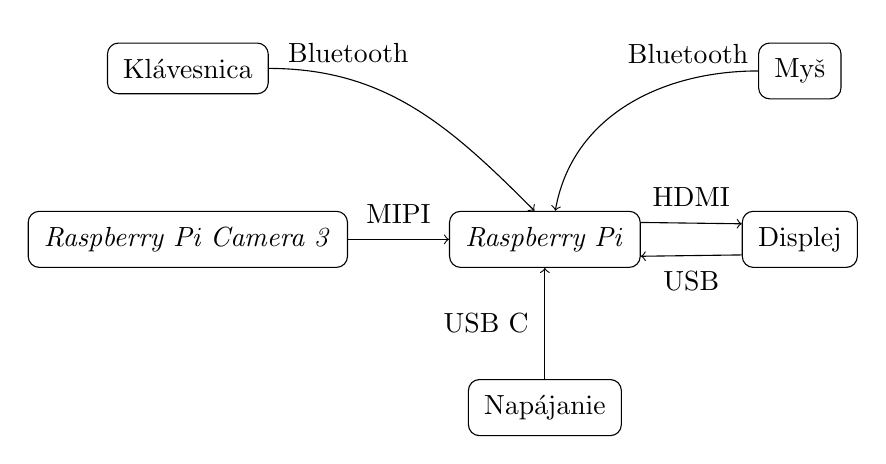
\begin{tikzpicture} [node distance=2.5cm, auto, inner sep=.2cm, rounded corners]
                \node (Pi) [draw, rectangle] at(0,0) {\emph{Raspberry Pi}};
                \node (Display) [right of=Pi, draw, rectangle, anchor=west] {Displej};
                \node (Camera) [left of=Pi, draw, rectangle, anchor=east] {\emph{Raspberry Pi Camera 3}};
                \node (Power) [below of=Pi, draw, rectangle, anchor=south] {Napájanie};
                \node (Keyboard) [above of=Camera, draw, rectangle, anchor=north] {Klávesnica};
                \node (Mouse) [above of=Display, draw, rectangle, anchor=north] {Myš};

                \draw[->] (Pi.10) -- (Display.165) node[midway, above] {HDMI};
                \draw[->] (Display.195) -- (Pi.350) node[midway, below] {USB};
                \draw[->] (Camera) -- (Pi) node[midway, above] {MIPI};
                \draw[->] (Power) -- (Pi) node[midway, left] {USB C};
                \draw[->] (Keyboard.east) to [out=. in=100] node[near start, above]{Bluetooth} (Pi.110);
                \draw[->] (Mouse.west) to [out=180, in=80] node[near start, above]{Bluetooth} (Pi.70);
            \end{tikzpicture}
            \caption{bloková schéma zariadenia}
        \end{figure}

\chapter{Tvorba datasetu}

    Správne naučenie modelov a ich schopnosť generalizovať z veľkej miery záleží na kvalite použitého datasetu (množiny dát). Tvorba datasetu je teda kľúčový krok pri práci so systémami strojového videnia.

    Cieľom pri tvorbe datasetu je zabezpečiť dostatočnú kvalitu a správnosť dát, dosiahnuť početne podobné zastúpenie každej triedy a správne reprezentovať rôznorodosť dát v rámci jednotlivých tried. Je vhodné aby boli vzorky získané pri rôznych podmienkach, podľa plánovaného použitia výsledného modelu.

    \section{Získavanie dát}

        Keďže táto práca nadväzuje na prácu \cite{Jurecka2021}, tvorí dataset v nej vytvorený základ pre ten použitý v tejto práci. Navyše bol rozšírený o niekoľko ďalších open source datasetov a vlastných anotovaných fotografii.

        Na tvorbu datasetu bol použitý program \emph{roboflow}, ktorý umožňuje načítavanie existujúcich datasetov, nahrávanie vlastných fotografii, anotáciu, spájanie dostupných datasetov, augmentácia datasetu a generovanie anotačných súborov rôznych formátov.

        Po pridaní všetkých častí datasetu a kontrole správnosti anotácie, boli počty inštancií jednotlivých tried:

        \begin{itemize}
            \item \textbf{vták}: 9047
            \item \textbf{dron}: 1190
            \item \textbf{helikoptéra}: 509
            \item \textbf{hmyz}: 249
            \item \textbf{lietadlo}: 845
        \end{itemize}

    \section{Úprava, rozdelenie a rozšírenie datasetu}

        Niektoré triedy sú reprezentované výrazne menším množstvom jednotlivých inštancii, čo je spôsobené nižšou dostupnosťou dát. Väčšina fotografii vtákov z vzdialenosti pri ktorej by mali byť detekované pochopiteľne obsahuje niekoľko desiatok jedincov, trieda vták je teda nadmerne zastúpená. Je možné tento problém čiastočne vyriešiť augmentáciou datasetu, čo program \emph{roboflow} umožňuje priamo pri generovaní novej verzie. V budúcnosti je vhodnejším riešením ďalšie rozšírenie datasetu o snímky s objektami aktuálne nedostatočne reprezentovaných tried.

        Aby bolo zabránené preučeniu modelu, musia byť dáta na ktorých je model učený rôzne od vylidačných a testovacích. Anotované obrazové dáta boli rozdelené do skupín s počtom:

        \begin{itemize}
            \item \textbf{trénovanie}: 2367
            \item \textbf{validácia}: 572
            \item \textbf{testovanie}: 290
        \end{itemize}

        Snímky boli predspracované upravením veľkosti na \(640 \times 640\) px a boli aplikované augmentácie, ktorými bol počet inštancií v trénovacej množine rozšírený na 7101:

        \begin{itemize}
            \item Rotácia \(-30^\circ\) až \(+30^\circ\)
            \item Zkosenie \(\pm 15^\circ\) vertikálne aj horizontálne
            \item Posun odtieňu \(-35^\circ\) až \(+35^\circ\)
            \item Zmena saturácie -25 \% až +25 \%
            \item Zmena expozície -20 \% až +20 \%
            \item Rozmazanie do 0,8 px
        \end{itemize}

    \section{Testovanie použiteľnosti datasetu}

    Použiteľnosť modelu bola testovaná naučením modelu typu \emph{Roboflow 3.0 Object Detection} priamo v aplikácii \emph{roboflow}, ktorý dosahoval úroveň presnosti 86.1 \% pri zvolenej variante modelu \emph{fast}. Pri dlhšom učení modelu určeného na reálne použitie sa dá predpokladať že dosiahnutá presnosť bude vyššia.

    Obrázok \ref{fig:roboflow_metrics} zobrazuje metriky presnosti naučeného modelu vypočítané v programe \emph{roboflow}, tak ako sa v ňom zobrazujú. Vypočítané metriky sú:

    \begin{itemize}
        \item \textbf{\ac{mAP}} \\ priemer priemerných presností za všetky triedy
        \item \textbf{Presnosť (Precision)} = \(\frac{TP}{TP + FP}\), značí s akou mieru správnej predikcie, v momente keď model nejakú hodnotu predikuje.
        \item \textbf{Senzitivita (Recall)} = \(\frac{TP}{TP + FN}\), na druhú stranu predstavuje pomer počtu správnych predikcii, ku počtu skutočne správnych hodnôt danej triedy.
    \end{itemize}

    \begin{figure}[H]
        \centering
        \includegraphics[width=.35\textwidth]{obrazky/roboflow/metrics.png}
        \caption{Metriky presnosti naučeného modelu v programe roboflow}
        \label{fig:roboflow_metrics}
    \end{figure}

    \begin{figure}[H]
        \centering
        \includegraphics[width=.8\textwidth]{obrazky/roboflow/train.png}
        \caption{Grafické zobrazenie priebehu učenia modelu roboflow}
    \end{figure}

    Výsledná vygenerovaná verzia datasetu je z programu exportovateľná v niekoľkých formátoch, napríklad pre učenie siete \ac{YOLO} alebo pre použitie s knižnicou \emph{tensorflow}. Pri exporte je stiahnutý komprimovaný priečinok obsahujúci obrazové dáta a anotáciu.

    \begin{figure}[H]
        \centering
        \includegraphics[width=.5\textwidth]{obrazky/roboflow/export.png}
        \caption{Exportovanie vytvoreného datasetu}
    \end{figure}

\chapter{Návrh softvéru}

    Pri návrhu a tvorbe aplikácie systému detekcie lietajúcich objektov bol kladený dôraz na:
    \begin{itemize}
        \item Spustiteľnosť a použiteľnosť na počítači
        \item Ovládateľnosť dotykovým panelom
        \item Modulárnosť a rozšíriteľnosť
        \item Spätná väzba a grafické zobrazenie výsledkov užívateľovi
        \item Možnosť používať, testovať a porovnávať rôzne metódy detekcie, klasifikácie a trasovania.
    \end{itemize}

    \section{Použitý jazyk a knižnice}

        Použitím programovacieho jazyka \emph{python}, bola získaná kompatibilita zo zariadeniami a operačnými systémami ktoré podporujú interpretér jazyka \emph{python}, teda hlavne \emph{Raspberry Pi} s nainštalovaným operačným systémom Raspberry Pi OS a osobné počítače, čo uľahčuje vývoj aplikácie a umožňuje jeho použitie na ľubovoľnom počítači.

        Na tvorbu grafického rozhrania bola použitá knižnica \ac{tkinter}. Tá umožňuje vytvárať grafické používateľské rozhranie priamo z kódu v jazyku \emph{python}. Obsahuje tiež objekty časovačov, vďaka ktorým je možné jednoducho a spoľahlivo ovládať kontinuálny beh aplikácie. Užívateľské rozhranie vytvorené knižnicou \ac{tkinter} je kompatibilné s ovládaním klávesnicou a myšou, aj dotykovým displejom.

        Knižnica \emph{OpenCV} obsahuje implementáciu množstva algorytmov spracovania obrazu a počítačového videnia. Umožňuje základné operácie s videom aj jednotlivými snímkami ako načítanie, ukladanie a zobrazovanie, pričom podporuje rôzne formáty obrazových dát. Sofistikovanejšie úlohy ktoré knižnica rieši zahrnujú detekciu, klasifikáciu, sledovanie pohybu. Knižnica \emph{OpenCV} je kompatibilná s viacerými programovacími jazykmi, vrátane jazyku \emph{python}.

    \section{Štruktúra aplikácie}

        Aplikácia je zložená z modulov reprezentujúcich jednotlivé implementované metódy detekcie, klasifikácie či trasovania alebo riadiacich modulov ovládajúcich tok dát medzi modulmi. Základnými typmi modulov tvoriacich aplikáciu sú:
        \begin{itemize}
            \item \textbf{Hlavná aplikácia} - existuje len jedna varianta, je zodpovedná za ovládanie systému, užívateľské rozhranie a súšťanie ostatných modulov. Pre každý z ďalších jednotlivých typov modulov je hlavnému modulu priradený zoznam existujúcich modulov daného typu, z ktorých si užívateľ môže vybrať ten aktívny, ktorý sa aktuálne použije na daný účel.
            \item \textbf{Poskytovateľ obrazu} - slúži na získavanie obrazových dát. Každý cyklus začína vyžiadaním nového obrazu od aktuálne zvoleného poskytovateľa obrazu hlavným modulom. Existujú dve varianty:
            \begin{itemize}
                \item \textbf{Video} - pri spustení aplikácia načíta všetky videá uložené v priečinku \path{./videos/} a pridá každému jeden objekt reprezentujúci dané video ako zdroj obrazu.
                \item \textbf{Kamera} - ak je v systéme nainštalovaná \emph{python} knižnica pre ovládanie kamery, je do zonamu poskytovateľov obrazu pridaný objekt reprezentujúci kameru.
            \end{itemize}
            \item \textbf{Detektor objektov} - po získaní aktuálneho obrazu je aplikovaný zvolený algorytmus detekcie. Detektoru je predaný obraz, jeho výstupom je zoznam rámikov oblastí v ktorých sa potenciálne nachádza objekt. V prípade zvolenia metódy detekcie a klasifikácie v jednom kroku je preskočený výber klasifikátora a výstupom je aj klasifikácia. 
            \item \textbf{Klasifikátor} - ak je zvolený algorytmus detekcie, sú oblasti s potenciálnym obsahom objektu predané klasifikátoru. Klasifikátor vráti hlavnému modulu zaradenie objektov do tried, po prípade označenie oblasti za pozadie. V hlavnej aplikácii je následne graficky zobrazené orámovanie a klasifikácia objektu.
            \item \textbf{Sledovač (Tracker)} - k ušetreniu výkonu je možne áplikovať detekciu a klasifikáciu len raz za určitý počet snímkov už a detekované a klasifikované objekty sledovať pomocou sledovačou z knižnice \emph{OpenCV}.
            \item \textbf{Tester výsledkov} - v prípade že je zvolené video ako zdroj obrazu a v priečinku \path{./video_annotation/} je pridaný \ac{csv} s rovnakým menom ako video obsahujúci správne orámovanie, je spustený testovací modul ktorý ohodnocuje detekciu a klasifikáciu podľa určenej správnej hodnoty zo súboru.
        \end{itemize}

        Jednotlivé moduly sú vytvárané dedením od abstraktnej triedy predstavujúcej rozhranie modulu s aplikáciou. Pre každý z typov modulu je pripravená jedna abstraktná rodičovská trieda, obsahujúca niektoré zdieľané premenné, ako je názov modulu a funkcie ktoré musí modul implementovať. Povinnou funkciou je napríklad funkcia vyžiadania si ďalšieho snímku pre modul poskytovateľa obrazu.

    \section{Implementácia}

        V aplikácii sú ako modul detekcie a klasifikácie aktuálne implementovaný model YOLO, pričom aplikácia automaticky pridá detekované naučené modely. Tie musia byť uložené v priečinku \path{./yolo/[model]/}, kde je \path{[model]} nahradené názvom modelu. v tomto priečinku je uložený model samotný v súbore \path{model.onnx} a \ac{csv} súbor so zoznamom názvov a farebných označení tried vo formáte \\
        \emph{"názov", "červená", "zelená", "modrá"} \\
        s názvom \path{classes.csv}. Aplikácia načíta všetky nájdené modely spolu s popisom tried a vloží ich do zoznamu detektorov.

    \section{Návrh grafického rozhrania}

        \ac{GUI} umožňuje intuitívne ovládanie aplikácie a zobrazovanie výsledkov detekcie, klasifikácie a sledovania.\linebreak Ovládanie jednotlivých modulov aplikácie je rozdelené do záložiek. Každá záložka umožňuje zvoliť ktorá z inštancii modulu každého z typov sa aktuálne používa.

        V ľavej časti obrazovky je zobrazený aktuálny snímok, s výstupom detekcie a klasifikácie. Zobrazujú sa v ňom orámovania detekovaných objektov, ich priradenie do tried a hodnotenie dôveryhodnosti klasifikácie. Ak existuje súbor s anotáciou správneho orámovania a klasifikácie pre aktuálne prehrávané video, sú zobrazené aj tie.

        V prvej záložke je užívateľovi umožnené zvoliť zdroj obrazu. Ak je aplikácia spustená na \emph{Raspberry Pi} a je nainštalovaná kižnica ovládania kamery, je do zoznamu zdrojov pridaná kamera. Pri spustení aplikácie sú načítané videá z priečinku \path{./videos} a sú zobrazené v zozname na záložke zdrojov spolu s kamerou. Kliknutím na názov zdroja je zdroj zvolený a užívateľovi sa z neho začne zobrazovať obraz.

        \begin{figure}[H]
            \centering
            \includegraphics[width=.7\textwidth]{obrazky/app/image_provider.png}
            \caption{Záložka na výber poskytovateľa obrazu}
        \end{figure}

        V druhej záložke výberu detektora si užívateľ vyberie metódu detekcie, alebo metódu súčasnej detekcie a klasifikácie, pri ktorej nie je použiteľný výber klasifikátoru na ďalšej záložke. Zároveň je na tejto záložke nastaviteľná perióda spúšťania detekcie, medzi snímkami na ktorých je detekcia spustená sa buď zobrazované ohraničenie nemení, alebo je akutalizované sledovačom.

        \begin{figure}[H]
            \centering
            \includegraphics[width=.7\textwidth]{obrazky/app/detector.png}
            \caption{Záložka na výber metódy detekcie objektov}
        \end{figure}

        V záložke sledovania objektov je umiestnený výber zo sledovačov implementovaných v knižnici \emph{OpenCV}. Sledovač je použitý na snímkoch medzi spustením detektcie.

        \begin{figure}[H]
            \centering
            \includegraphics[width=.7\textwidth]{obrazky/app/tracker.png}
            \caption{Záložka na výber metódy sledovania objektov}
        \end{figure}

        Posledná záložka obsahuje menu z možnosťou zapnúť a vypnúť zobrazenie detekcie konkrétnych tried objektov. 

        \begin{figure}[H]
            \centering
            \begin{tikzpicture}[node distance=.5\textwidth]
                \node (image1) {\includegraphics[width=.45\textwidth]{obrazky/app/class_settings_1.png}};
                \node (image2) [right of=image1] {\includegraphics[width=.45\textwidth]{obrazky/app/class_settings_2.png}};
            \end{tikzpicture}
            \caption{Záložka na výber detekovaných tried}
        \end{figure}